% README architecture: extracted from the manuscript method diagram without its panel label.
\documentclass[tikz,border=1.44mm]{standalone}
\usepackage[T1]{fontenc}
\usepackage{helvet,amsmath,amssymb}
\renewcommand{\familydefault}{\sfdefault}
\usetikzlibrary{arrows.meta,calc,positioning}
\definecolor{base}{HTML}{B64342}
\definecolor{heat}{HTML}{0F4D92}
\definecolor{control}{HTML}{767676}
\definecolor{warm}{HTML}{FFB000}
\definecolor{tauA}{HTML}{3775BA}\definecolor{tauB}{HTML}{42949E}\definecolor{tauC}{HTML}{9A4D8E}
\tikzset{flow/.style={-{Stealth[length=1.6mm]},line width=.55pt,draw=black!65},
 block/.style={draw=black!40,line width=.45pt,fill=white,align=center,minimum height=.65cm,inner sep=4pt,font=\fontsize{8bp}{9.6bp}\selectfont},
 lab/.style={font=\fontsize{8bp}{9.6bp}\selectfont,align=center},
 smalllab/.style={font=\fontsize{8bp}{9.6bp}\selectfont,align=center}}
\begin{document}
\pagecolor{white}
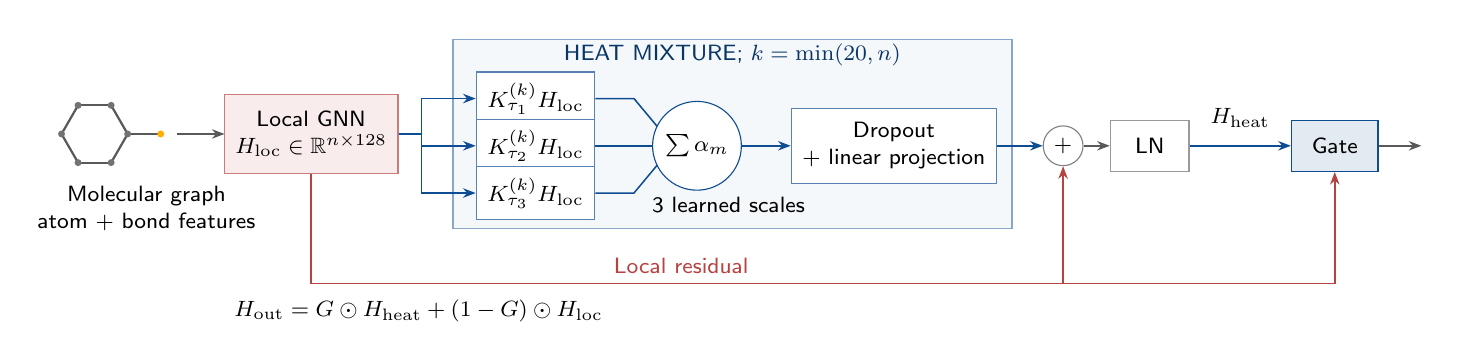
\begin{tikzpicture}[x=1cm,y=1cm,font=\fontsize{8bp}{9.6bp}\selectfont]
\path[use as bounding box] (0,-.55) rectangle (18,-4.45);
% molecular connectivity; no atom-wise experimental measurement is implied
\begin{scope}[shift={(.85,-1.9)},scale=.42]
\foreach \i in {0,...,5}{\coordinate (v\i) at (60*\i:1);}
\foreach \i/\j in {0/1,1/2,2/3,3/4,4/5,5/0}{\draw[black!65,line width=.8pt] (v\i)--(v\j);}
\draw[black!65,line width=.8pt] (v0)--(2,0);
\foreach \i in {0,...,5}{\fill[black!55] (v\i) circle (3pt);}
\fill[warm] (2,0) circle (3pt);
\end{scope}
\node[smalllab,anchor=west] at (0,-2.85) {Molecular graph\\atom + bond features};
\draw[flow] (1.9,-1.9)--(2.5,-1.9);
\node[block,fill=base!10,draw=base!70,minimum width=2.1cm,minimum height=1cm] (local) at (3.6,-1.9) {Local GNN\\$H_{\mathrm{loc}}\in\mathbb{R}^{n\times128}$};
\draw[heat!50,line width=.5pt,fill=heat!4] (5.4,-.7) rectangle (12.5,-3.1);
\node[smalllab,text=heat!70!black] at (8.95,-.9) {HEAT MIXTURE; $k=\min(20,n)$};
\foreach \j/\yy in {1/-1.45,2/-2.05,3/-2.65}{
 \node[block,draw=heat!70,minimum width=1.5cm,minimum height=.46cm] (k\j) at (6.45,\yy) {$K_{\tau_\j}^{(k)}H_{\mathrm{loc}}$};
 \draw[flow,draw=heat] (local.east)--(5,-1.9)|-(k\j.west);
 \draw[flow,draw=heat] (k\j.east)--(7.7,\yy)--(8.2,-2.05);
}
\node[circle,draw=heat,fill=white,inner sep=3pt] (sum) at (8.5,-2.05) {$\sum\alpha_m$};
\node[smalllab] at (8.9,-2.8) {3 learned scales};
\node[block,draw=heat!70,minimum width=2.15cm,minimum height=.95cm] (proj) at (11,-2.05) {Dropout\\+ linear projection};
\draw[flow,draw=heat] (sum.east)--(proj.west);
\node[circle,draw=black!50,fill=white,inner sep=2pt] (add) at (13.15,-2.05) {$+$};
\draw[flow,draw=heat] (proj.east)--(add.west);
\draw[flow,draw=base] (local.south)--(3.6,-3.8)--(13.15,-3.8)--(add.south);
\node[smalllab,text=base] at (8.3,-3.57) {Local residual};
\node[block,minimum width=1cm] (ln) at (14.25,-2.05) {LN};
\draw[flow] (add.east)--(ln.west);
\node[block,fill=heat!12,draw=heat,minimum width=1.1cm] (gate) at (16.6,-2.05) {Gate};
\draw[flow,draw=heat] (ln.east)--node[midway,above=3pt,smalllab] {$H_{\mathrm{heat}}$}(gate.west);
\draw[flow,draw=base] (13.15,-3.8)--(16.6,-3.8)--(gate.south);
\draw[flow] (gate.east)--(17.7,-2.05);
\node[smalllab,anchor=west] at (2.5,-4.15) {$H_{\mathrm{out}}=G\odot H_{\mathrm{heat}}+(1-G)\odot H_{\mathrm{loc}}$};
\end{tikzpicture}
\end{document}
